%!TEX root = ../dokumentation.tex

\section{Entwickeltes System}


\subsection{Android Client}

\subsubsection{Activities}

\begin{figure}[H]
	\centering
	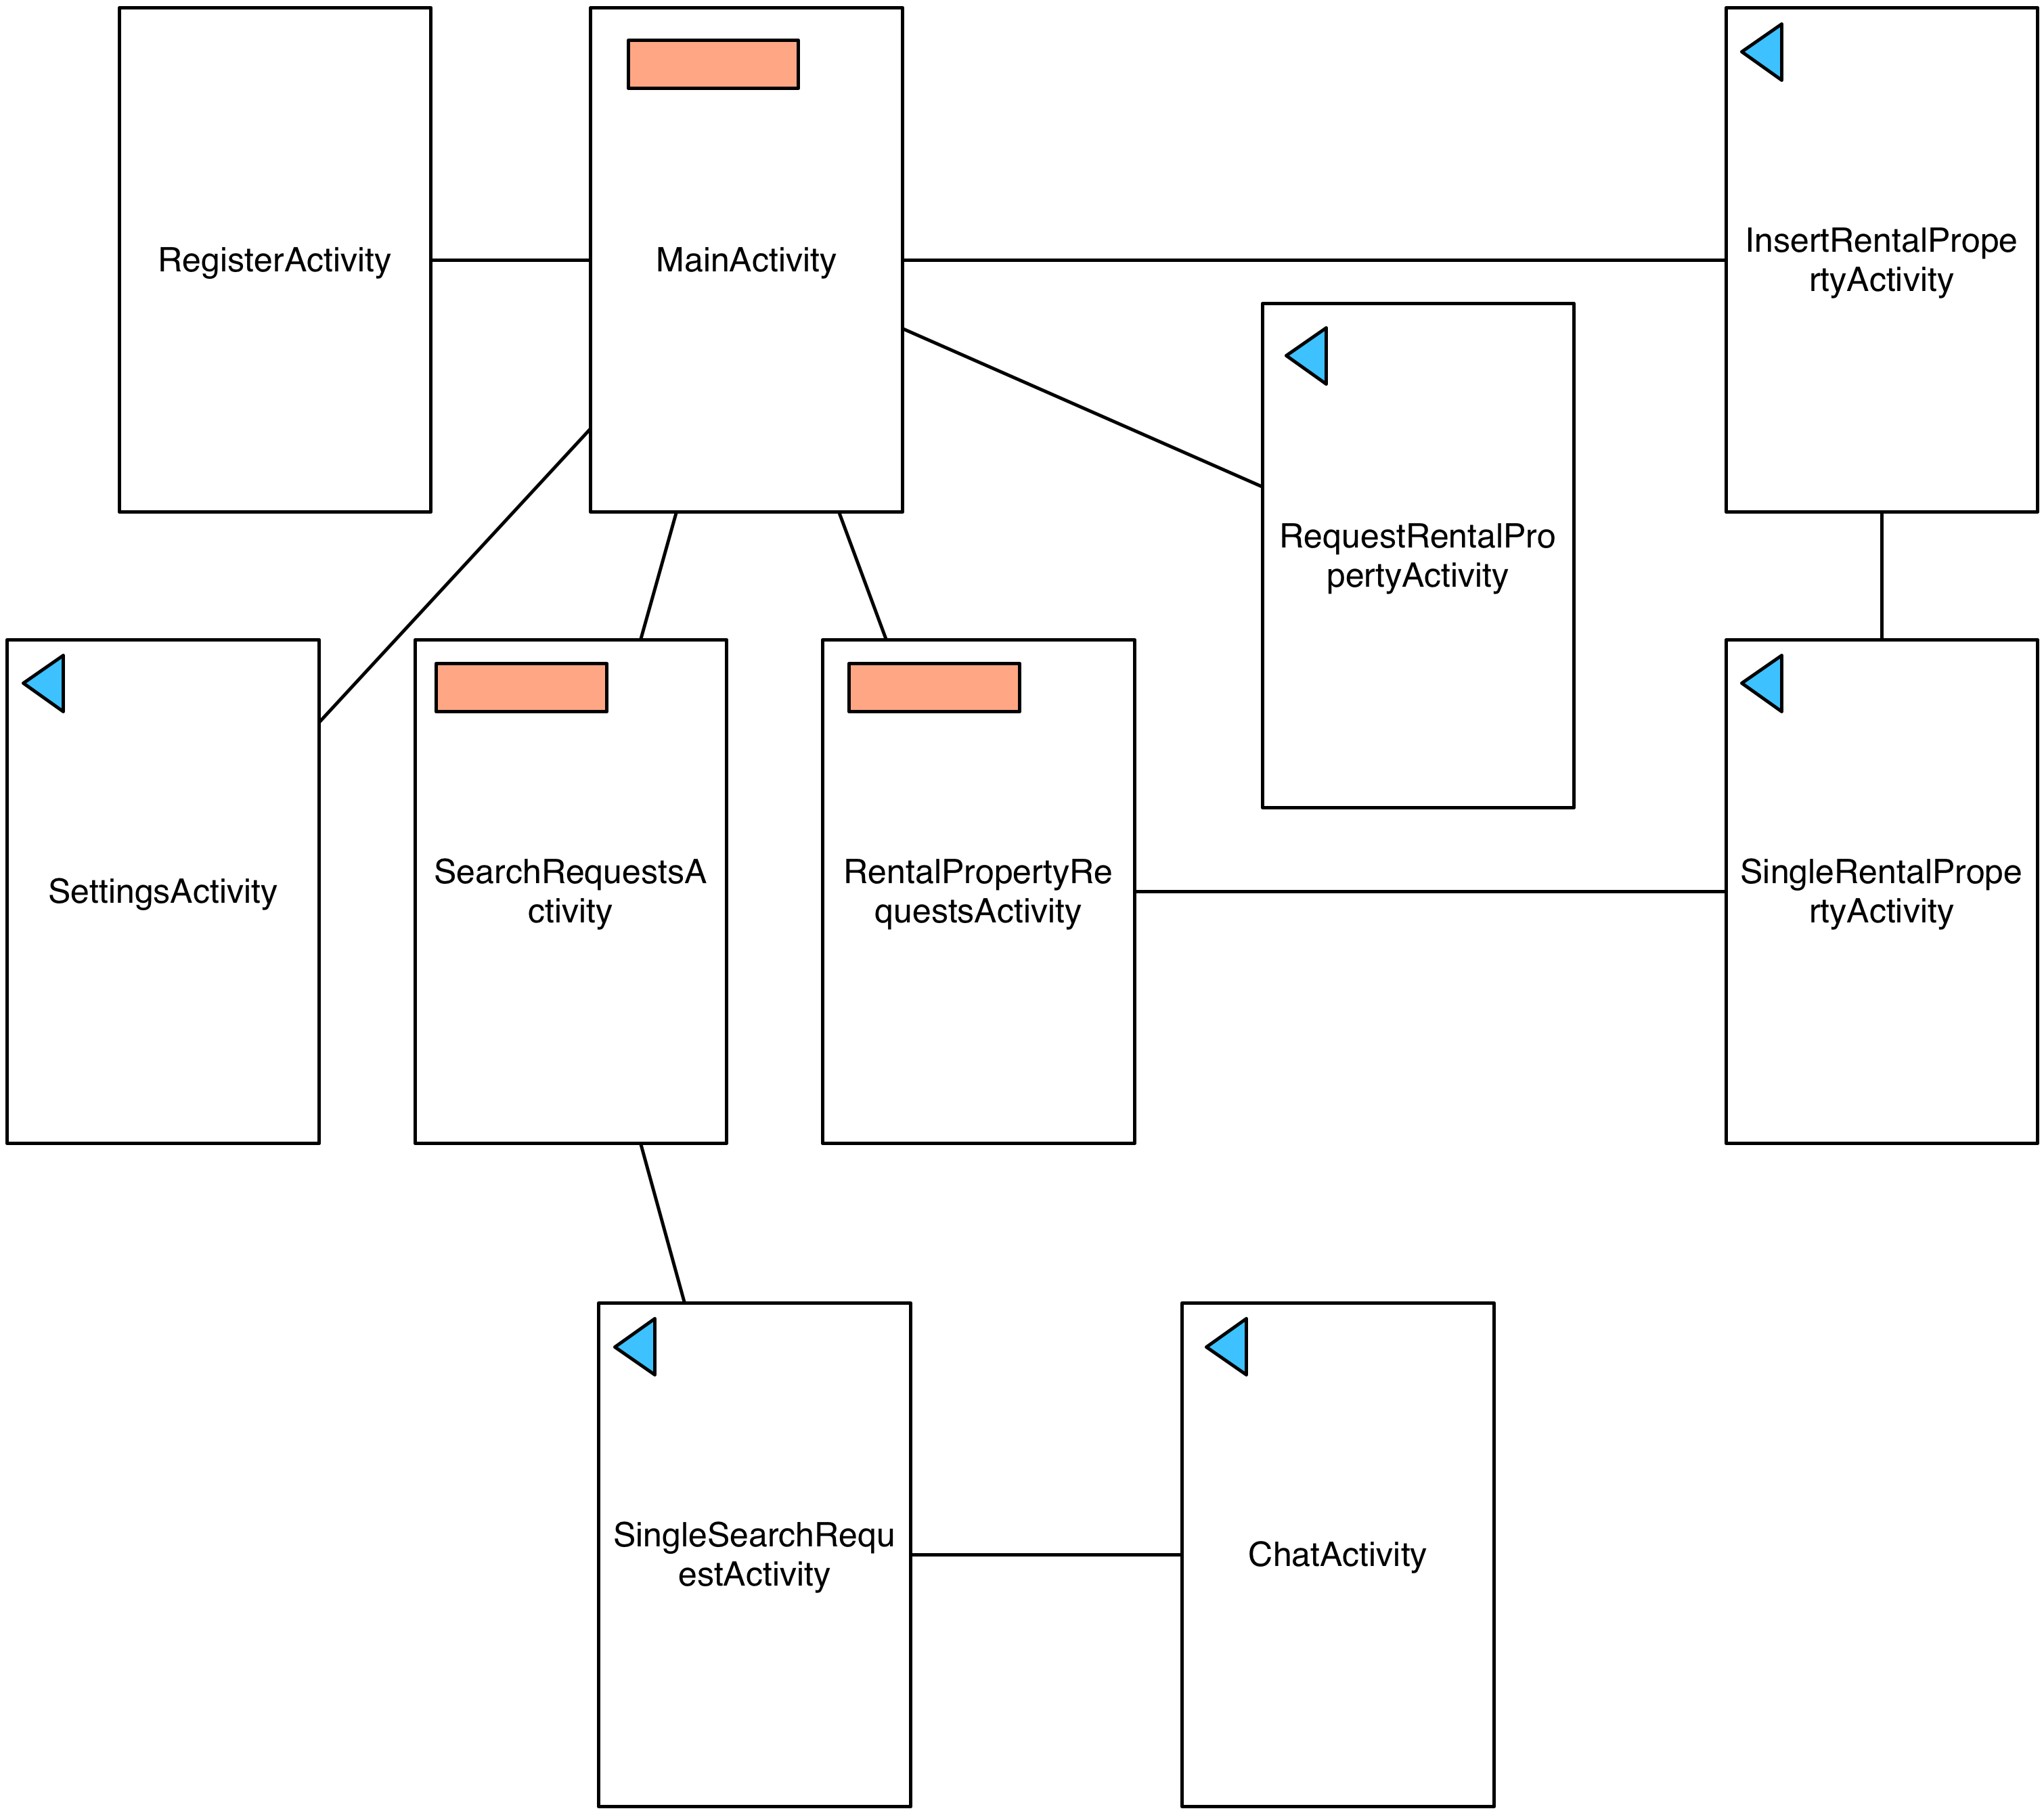
\includegraphics[width=0.85\textwidth]{./images/activitiesoverview.png}
	\caption{Übersicht der Activities und Navigationselementen}
	\label{fg:activitiesoverview}
\end{figure}

Activities sind die Komponenten, die dem Benutzer visuell Interaktionen anbieten können. Die Activities sollten untereinander verbunden werden, um so einen gewissen Workflow zu garantieren und „Sackgassen“ zu vermeiden.

\subsubsection{Datenbank}

Wie im Proof-of-Concept „Lokale Datenbankanbindung“ (vgl Kapitel 3.2.4) bereits dokumentiert, wird das System mit dem Datenbanksystem SQLite arbeiten. Im Folgenden wird nun auf die endgültige Implementierung im System eingegangen.

Zunächst wurde eine abstrakte Klasse \texttt{Table} entwickelt (Code \ref{ls:abstracttableclass}), welches nichts anders macht, als den Datenbanknamen sowie die aktuelle Datenbankversion beinhaltet. Die Klasse erweitert die Klasse \texttt{SQLiteOpenHelper}.

\begin{lstlisting}[label=ls:abstracttableclass,caption=Abstrakte Klasse \texttt{Table}]
public abstract class Table extends SQLiteOpenHelper {
	private static final String DATABASE_NAME = "data.db";
	private static final int DATABASE_VERSION = 1;

	public Table(Context context) {
		super(context, DATABASE_NAME, null, DATABASE_VERSION);
	}
}
\end{lstlisting}

Der Ausschnitt (Code \ref{ls:userstableclass}) der Implementation der \texttt{UserTable} demonstriert die Vererbung der Klasse \texttt{Table}.

\begin{lstlisting}[label=ls:userstableclass,caption=Ausschnitt aus der Klasse \texttt{UsersTable}]
public class UsersTable extends Table {

	public static final String TABLE_NAME = "users";
	public static final String COLUMN_NAME_ID = "id";
	public static final String COLUMN_NAME_USER_NAME = "name";

	private static final String TABLE_CREATE =
		"CREATE TABLE " + TABLE_NAME + " (" +
			COLUMN_NAME_ID + " integer primary key autoincrement," +
			COLUMN_NAME_USER_NAME + " text NOT NULL" +
		");";

	private static final String TABLE_DROP =
		"DROP TABLE IF EXISTS " + TABLE_NAME;

	public UsersTable(Context context) {
		super(context);
	}

	public void onCreate(SQLiteDatabase db) {
		db.execSQL(TABLE_CREATE);
	}
}
\end{lstlisting}

Hierbei hat sich als hilfreich erwiesen, Tabellenspezifische Angaben wie Tabellenname oder Spaltenamen in Konstanten auszulagern, um diese wiederverwertbar zu gestalten. Dies spiegelt sich zum Beispiel bei einem Insert-Befehl wieder (Code \ref{ls:userstableinsert}).

\begin{lstlisting}[label=ls:userstableinsert,caption=Exemplarisches Insert in die „UsersTable“]
UsersTable usersTable = new UsersTable(this);
SQLiteDatabase usersTableDb = usersTable.getWritableDatabase();

ContentValues values = new ContentValues();
values.put(UsersTable.COLUMN_NAME_ID, id);
values.put(UsersTable.COLUMN_NAME_USER_NAME, username);

long userId = usersTableDb.insert(
	UsersTable.COLUMN_NAME_ID,
	UsersTable.COLUMN_NAME_USER_NAME,
	values);
\end{lstlisting}

\subsubsection{Google Cloud Messaging}

Die Implementierung der GCM Schnittstelle hatte sich bereits im Proof-of-Concept als kompliziert erwiesen. Im Entwicklungssystem wurde dies wiederum bestätigt.

Ein aufgetretenes Problem war das fehlende Auslösen des Hintergrundprozesses, welches es unmöglich machte, die Push Notifcations zu bearbeiten. Eine Fehlerausgabe suchten wir vergeblich. Nach längeren Debugging wurde der recht banale Fehler gefunden: Es gab eine Komplikation bei den Berechtigungen in der Datei \texttt{AndroidManifest.xml} (Code \ref{ls:androidmanifest}).

\begin{lstlisting}[label=ls:androidmanifest,caption=Auszug aus der AndroidManifest.xml,language=xml]
<?xml version="1.0" encoding="utf-8"?>
<manifest xmlns:android="http://schemas.android.com/apk/res/android"
    package="de.fhkoeln.gm.findyourcamp.app"
    android:versionCode="1"
    android:versionName="1.0" >

    <permission android:name="de.fhkoeln.gm.findyourcamp.app.permission.C2D_MESSAGE" android:protectionLevel="signature" />
    <uses-permission android:name="de.fhkoeln.gm.findyourcamp.app.permission.C2D_MESSAGE" />
\end{lstlisting}

Der Fehler lag darin, dass der Wert für \texttt{package} nicht dem Präfix in Zeile 7 und 8 entsprach. Der korrekte Name der Berechtigung baut sich somit über \texttt{\{Paketname\}.permission.C2D\_MESSAGE} auf.


\subsubsection{Message Broker}

Über den GCM Dienst werden alle Daten als Nachrichten transportiert. Die einzelnen Nachrichten müssen aus diesem Grund einer eindeutigen Aktion zugeordnert werden können. Diese Aktion bestimmt dann die weitere Verarbeitung der Nachricht. Die Aktion wird im Payload der Nachricht unter dem Key \texttt{action} aufgeführt. Der Message Broker prüft dieses Feld und routet die Nachricht an den jeweiligen Controller weiter. Bei Bedarf kann dieser auch Nachrichten zunächst sammeln und als Ganzes weiterleiten.

Der Message Broker kommt jeweils in der Clientanwendung sowie in der Serveranwendung zum Einsatz. Das folgende Beispiel (Code \ref{ls:messagebroker}). zeigt einen Ausschnitt des Message Broker, welcher im Client zum Einsatz kommt.

\begin{lstlisting}[label=ls:messagebroker,caption=Intent Service mit Message Broker]
public class GcmIntentService extends IntentService {

    public GcmIntentService() {
        super("GcmIntentService");
    }

    @Override
    protected void onHandleIntent(Intent intent) {
        Bundle extras = intent.getExtras();
        GoogleCloudMessaging gcm = GoogleCloudMessaging.getInstance(this);
        String messageType = gcm.getMessageType(intent);

        if (!extras.isEmpty()) {  // has effect of unparcelling Bundle
            if (GoogleCloudMessaging.MESSAGE_TYPE_SEND_ERROR.equals(messageType)) {
               // ...
            } else if (GoogleCloudMessaging.MESSAGE_TYPE_DELETED.equals(messageType)) {
               // ...
            } else if (GoogleCloudMessaging.MESSAGE_TYPE_MESSAGE.equals(messageType)) {
            	MessageBroker mb = new MessageBroker(extras);
            	mb.handleRequest();
            }
        }
        GcmBroadcastReceiver.completeWakefulIntent(intent);
    }
}

public class MessageBroker {

	public static final int ACTION_RESPONSE_USER_REGISTER  = 1;
	public static final int ACTION_RESPONSE_SEARCH_REQUEST = 2;

	Bundle data;

	public MessageBroker(Bundle data) {
		this.data = data;
	}

	public void handleRequest() {
		int action = (Integer) data.get("action");

		switch (action) {
			case ACTION_RESPONSE_USER_REGISTER:
				// ...
				break;
			case ACTION_RESPONSE_SEARCH_REQUEST:
				// ...
				break;
			default:
				Logger.error("Unsupported action: " + action);
				break;
		}
	}
}
\end{lstlisting}

Dem Message Broker wird der Payload übergeben. Dieser prüft zunächst das Feld \texttt{action}, welches mit einem int-Wert belegt ist und leitet dann die weitere Verarbeitung ein.

\subsection{Serveranwendung}

\subsubsection{Datenbank}

Für die Speicherung von Daten wurden die Datenbanksysteme SQLite, MySQL und MongoDB in Erwägung gezogen. Die Einbindung in Java geschieht dabei über Treiber. Der zugehörige Treiber  muss dafür geladen werden und dem Projekt als Bibliothek zugewiesen werden.

Bei der Implementierung ist auf einen Fehler einzugehen: Das Laden des Laden des Treibers wird über einen dynamischen Klassenaufruf gesteuert. In den jeweiligen Anleitungen war folgender Schnipsel (Code \ref{ls:wrongdriveruse}) zu sehen (vgl. Verbindung mit MySQL über die Schnittstelle DriverManager\footnote{\url{http://dev.mysql.com/doc/refman/5.1/de/connector-j-usagenotes-basic.html\#connector-j-usagenotes-connect-drivermanager}, zuletzt gesichtet am 13. Januar 2014})

\begin{lstlisting}[label=ls:wrongdriveruse,caption=Fehlerhafter dynamischer Klassenaufruf]
try {
	Class.forName("com.mysql.jdbc.Driver").newInstance();
} catch (Exception ex) {
	// Fehler behandeln
}
\end{lstlisting}

Die Nutzung des Schnipsels gab jedoch nicht das gewünschte Ergebnis aus, genauer gesagt gar nichts. Die Lösung des Problems bestand darin, den Aufruf \textit{.newInstance()} zu entfernen (Code \ref{ls:correctdriveruse}).

\begin{lstlisting}[label=ls:correctdriveruse,caption=Korrekter dynamischer Klassenaufruf]
try {
	Class.forName("com.mysql.jdbc.Driver")
} catch (Exception ex) {
	// Fehler behandeln
}
\end{lstlisting}

In der folgenden Übersicht werden die drei Datenbanksysteme anhand eines Beispiels - anlegen einer Tabelle und einfügen eines Wertes - gegenübergestellt:

\paragraph{SQLite}

Treiber: \url{https://bitbucket.org/xerial/sqlite-jdbc}
\begin{lstlisting}[label=ls:sqliteexample,caption=Exemplarische Darstellung der Nutzung des SQLite Treibers]
Class.forName("org.sqlite.JDBC");
Connection connection = DriverManager.getConnection("jdbc:sqlite:findyourcamp.db");
Statement statement = con.createStatement();
statement.executeUpdate("drop table if exists users");
statement.executeUpdate("create table users (id integer, name string)");
statement.executeUpdate("insert into person values(1, 'max')");
\end{lstlisting}

\paragraph{MySQL}

Treiber: \url{http://dev.mysql.com/downloads/connector/j/}
\begin{lstlisting}[label=ls:mysqlexample,caption=Exemplarische Darstellung der Nutzung des MySQL Treibers]
Class.forName("com.mysql.jdbc.Driver");
Connection connection = DriverManager.getConnection("jdbc:mysql://localhost:3306/findyourcamp", "username", "password");
Statement statement = con.createStatement();
statement.executeUpdate("drop table if exists users");
statement.executeUpdate("create table users (id int, name text)");
statement.executeUpdate("insert into person values(1, 'max')");
\end{lstlisting}

\paragraph{MongoDB}

Treiber: \url{http://docs.mongodb.org/ecosystem/drivers/java/}
\begin{lstlisting}[label=ls:mongoexample,caption=Exemplarische Darstellung der Nutzung des MongoDB Treibers]
MongoClient mongoClient = new MongoClient();
DB db = mongoClient.getDB("findyourcamp");
DBCollection collection = db.getCollection("users");
collection.insert(new BasicDBObject("name", "max"));
\end{lstlisting}

SQLite kennen wir schon aus der Entwicklung der Android Applikation. Als weiteres relationales Datenbanksystem ist MySQL gewählt worden. Der Unterschied zwischen beiden System liegt darin, dass MySQL auf eine exterene Datenbasis setzt, wo SQLite sich direkt in die Anwendungen integrieren lässt. MongoDB hingegen kommt aus der NoSQL Sparte. Die Daten werden im JSON Format hinterlegt, wodurch das System gut skalierbar ist. Die Nachteile liegen allerdings in der fehlenden Relationen oder einer Volltext-Suche.

In den Tests (Code \ref{ls:performancetest}) zeigte sich außerdem, dass NoSQL, sowie auch SQLite, um 50\% langsamer als die MySQL Implementation war.

\begin{lstlisting}[label=ls:performancetest,caption=Perfomancetest zwischen MySQL und SQLite,language=bash]
$ time java -jar test_sqlite.jar
java -jar test_sqlite.jar 2,24s user 0,46s system  97% cpu 2,760 total
$ time java -jar test_mysql.jar
java -jar test_mysql.jar  1,47s user 0,17s system 133% cpu 1,225 total
\end{lstlisting}

Da der Zeitfaktor doch eine große Rolle in unserem System spielt, wurde entschieden für die Serveranwendung auf MySQL zu setzen. Jedoch sollte, sofern es die Zeit zulässt, eine gewisse Abstraktion geschaffen werden, wodurch ein späteres Ändern des Datenbanksystems durchführbar ist.

\subsection{Matching Algorithmus}

In Konzept wurde bereits kurz darauf eingegangen: Um den Vermieter vor einer Flut an Mietanfragen zu schützen, bekommt dieser nur eine Benachrichtigung bei relevanten Anfragen. Wann ist eine Anfrage releveant?

\begin{enumerate}
	\item \textbf{Ort:} Der Ort wird über einen serverseitigen Abgleich auf Relevanz geprüft. Zur Erinnerung: In den Datenbanken auf dem Server werden nur die Orte mit der jeweiligen Vermieter ID gespeichert. Entspricht ein Ort der Anfrage so wird dem Device des Vermieters die Anfrage weitergeleitet.
	\item \textbf{Gruppengröße:} Die Gruppengröße dient als Grundlage für den nächsten Abgleich. Ist die geforderte Gruppengröße kleiner oder gleich der verfügbaren Größe, ist das Objekt als relevant zu betrachten.
	\item \textbf{Preis:} Bevor die Ausstattung geprüft wird, wird zunächst ein Abgleich zwischen gewünschter und geforderter Preis durchgeführt. Das Objekt ist weiterhin relevant, wenn der gewünschte Preis dem des Vermieters entspricht.
	\item \textbf{Ausstattung:} Die Ausstattungsmerkmale werden als Boolean Werte verarbeitet. Dadurch ergeben sich nur die Werte 1 und 0.
	Die Relevanz kann daher auf Basis des Skalarproduktes ermittelt werden. Vektor A entspricht dabei den Daten des Vermieters, Vektor B dem des potentiellen Mieters. Wünscht der Mieter 4 Ausstattungsmerkmale und das Skalarprodukt ergibt zwei oder mehr, so ist das Objekt relevant und der Vermieter wird endgültig über die Anfrage benachrichtigt.
\end{enumerate}

Der relevante Code hierfür befindet sich in der Klasse \texttt{LocationMatch} im Paket \texttt{de.fhkoeln.gm.findyourcamp.server.matching} für das Server-Matching und das Client-Matching wird in der Klasse \texttt{RentalPropertyMatch} im Paket \texttt{de.fhkoeln.gm.findyourcamp.app.matching} sichtbar.

